\documentclass[14pt, a4paper]{extreport}
\usepackage[utf8]{inputenc}
\usepackage[english,russian]{babel}
\usepackage[left=2.5cm,right=1.5cm,
    top=2cm,bottom=3cm,bindingoffset=0cm]{geometry}
\usepackage{indentfirst}

\usepackage[pdftex]{graphicx}
\DeclareGraphicsExtensions{.pdf,.png,.jpg}
\graphicspath{{pictures/}}
\usepackage{tocloft}
\setlength{\cftbeforetoctitleskip}{-2em}

\usepackage{misccorr}
\usepackage{graphicx}
\usepackage{amsmath}
\usepackage{amssymb}
\usepackage{breqn}
\renewcommand{\baselinestretch}{1.5}
\usepackage{ragged2e}
\usepackage{enumitem}
\setlist{nolistsep}
\justifying

\makeatletter
\renewcommand\@biblabel[1]{#1.\hfil}
\makeatother

\begin{document}
\begin{titlepage}

\begin{center}
Министерство науки и высшего образования Российской Федерации\\ 
\vspace{5mm}
Федеральное государственное автономное образовательное учреждение высшего образования\\
Национальный исследовательский Нижегородский государственный университет им. Н.И. Лобачевского\\
\vspace{1cm}
Институт информационных технологий, математики и механики\\
\vspace{5cm}
\textbf{\large Отчет по лабораторной работе} \\
\vspace{8mm}
\textbf{\Large «Выделение ребер на изображении с использованием оператора Собеля»} \\

\end{center}

\newlength{\ML}
\settowidth{\ML}{«\underline{\hspace{0.7cm}}» \underline{\hspace{2cm}}}

\begin{flushright}
\textbf{ Выполнил:}\\
студент группы 381706-1\\
Голованова Е. А.\\
\end{flushright}
\begin{flushright}
\textbf{Проверил:}\\
доцент кафедры МОСТ,\\
кандидат технических наук\\
Сысоев А. В. \\
\end{flushright}
\vfill 
\begin{center}
 Нижний Новгород\\
 2020 г.
\end{center}
\end{titlepage}
\setcounter{page}{2}
\tableofcontents
\newpage 

\section*{Введение}
\addcontentsline{toc}{section}{Введение}

Оператор Собеля - дискретный дифференциальный оператор, вычисляющий приближенные значения производных разного порядка для функции яркости пикселей. Наиболее часто используется для определения ребер объектов на изображении.

Данный оператор основан на операции свертки изображения. В простейшем случае свертка вычисляется с ядрами \begin{math}G_x, G_y\end{math}, обеспечивающими вычисление первых производных по направлениям:

\begin{equation}
G_x=
\left[
  \begin{array}{ccc}
    -1 & 0 & 1 \\
     -2 & 0 & 2 \\
     -1 & 0 & 1\\
  \end{array}
\right]
,G_y=
\left[
  \begin{array}{ccc}
    -1 & -2 & -1 \\
     0 & 0 & 0 \\
     1 & 2 & 1\\
  \end{array}
\right]
\end{equation}

Оператор Собеля используется для приближенного вычисления градиента функции интенсивности пикселей. Применение оператора  \begin{math}G_x\end{math}  позволяет определить приближенное значение первой частной производной изменения интенсивности в горизонтальном направлении, \begin{math}G_y\end{math} – в вертикальном. На основании данной информации можно вычислить магнитуду градиента для пикселя с координатами \begin{math}(i,j)\end{math} согласно следующей формуле:  \begin{equation}|G^{i,j}|=\sqrt{(G^{i,j}_x)^2+(G^{i,j}_y)^2}\end{equation}
\newpage 

\section*{Постановка задачи}
\addcontentsline{toc}{section}{Постановка задачи}

В данной лабораторной работе можно выделить несколько задач:
 \begin{enumerate} 
 \item Разработать последовательный алгоритм оператора Собеля и написать автоматические тесты с использованием Google C++ Testing Framework для него.
 \item Разработать параллельный алгоритм оператора Собеля при помощи технологии OpenMP и написать автоматические тесты с использованием Google C++ Testing Framework для него.
 \item Аналогично для технологии TBB.
 \item Аналогично для технологии std::threads.
 \item Провести вычислительные эксперименты для каждой технологии и сравнить результаты.
 \end{enumerate}


\newpage 
\section*{Описание алгоритма}
\addcontentsline{toc}{section}{Описание алгоритма}
В самом алгоритме можно выделить две части: операция свертки и вычисление результата. 

Операция свертки происходит следующим образом. Изображение можно представить в виде матрицы чисел, которые находятся в промежутке от 0 до 255. По этой матрице "скользит" ядро, выполняя поэлементное умножение для той части данных, которую сейчас покрывает. Результаты переумножений ячеек суммируются.

В операторе Собеля вычисления ведут два ядра, поэтому после суммирования результат каждого возводится в квадрат, эти вычисления суммируются, и от результата берут квадратный корень. Далее оба этапа повторяются для каждой локации, по которой проходит ядро.

Скольжение ядра "обрезает" исходную матрицу чисел по краю, то есть краевые пиксели теряются из-за того, что ядро не может распространяться за пределы края. Во избежание этого добавляется подготовительный этап: окружение матрицы краевым полем, значения которого нули.
\newpage 

\section*{Описание структуры программы}
\addcontentsline{toc}{section}{Описание структуры программы}

Программа разработана в виде класса \verb|image|. Этот класс имееет три приватных поля: два поля типа int \verb|width и height|, обозначающие соотвественно ширину и высоту изображения, и поле типа vector \verb|matrix|, в котором находятся значения пикселей изображения (то есть типа int).

Для удобства были разработаны два конструктора данного класса, функция, позволяющая задавать матрицу рандомными числами, функция, позволяющая получать значения матрицы, и функции, реализующие оператор Собеля.

Сам проект состоит из четырех файлов: 
\begin{itemize}
\item sobel.h - создание класса и прототипы функции
\item sobel.cpp - реализация конструкторов и функций
\item main.cpp - Google-тесты
\item CMakeLists.txt
\end{itemize}

\newpage 

\section*{Схема распараллеливания}
\addcontentsline{toc}{section}{Схема распараллеливания}

\subsection*{OpenMP}
\addcontentsline{toc}{subsection}{OpenMP}

Вся реализация оператора Собеля состоит из нескольких вложенных циклов (два из них идут по ширине и высоте исходной матрицы, другие два - по элементам подматрицы, на которой находится ядро). В таком случае для распараллеливания удобно пользоваться директивой \verb|pragma omp parallel for|. Эта директива сообщает, что при выполнении цикла for в параллельном регионе итерации цикла должны быть распределены между потоками группы.

\subsection*{TBB}
\addcontentsline{toc}{subsection}{TBB}

В этой технологии распараллеливание происходит при помощи шаблонной функции. Она имеет вид:
\begin{verbatim}
tbb::parallel_for(tbb::blocked_range<int>{0, width}, 
		[&](const tbb::blocked_range<int>& rows)
\end{verbatim}

Первый параметр обозначает итерационное пространство - класс специального вида, задающий количество итераций (в данном случае количество итераций соответствует ширине матрицы). Второй - функтор - класс специального вида, который выполняет необходимые вычисления.

\subsection*{std::threads}
\addcontentsline{toc}{subsection}{std::threads}

Для использования данной технологии необходимо создать объекты\\
\verb|std::thread|. При этом под каждый поток необходим свой объект класса. После этого происходит распределение итераций между потоками: делим ширину матрицы на количество потоков - такова будет порция для каждого объекта . После этого каждый поток совершает вычисления и получает свой пиксель. В случае если остаток от деления не равен нулю, то вычисления совершает последний поток.

Для корректности выполнения используем функцию \verb|std::thread::join|, чтобы дождаться завершения всех потоков.
\newpage

\section*{Результаты экспериментов}
\addcontentsline{toc}{section}{Результаты экспериментов}

Конфигурация системы:
\begin{itemize}
\item Процессор: AMD A8-9600 RADEON R7, 10 COMPUTE CORES 4C+6G 3.10 GHz;
\item Оперативная память: 16Gb;
\item ОС: Microsoft Windows 10 Домашняя;
\item Количество ядер - 4
\end{itemize}

Эксперименты проходят на матрице постоянного размера 10000*10000. В данной лабораторной работе рассматривается эффективность при различных технологиях на разном количестве потоков. Время измеряется в секундах.

\begin{figure}[h]
\center{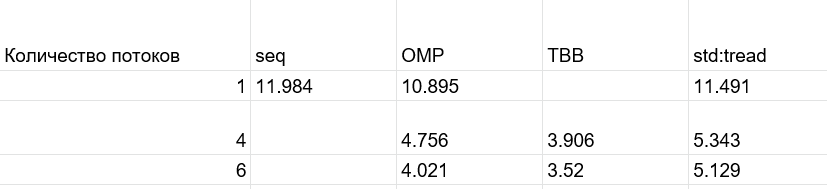
\includegraphics[scale=0.7]{res.png}}
\caption{Таблица значений}
\label{fig:image}
\end{figure}

На одном потоке время работы паралельного алгоритма схоже с временем работы последовательного алгоритма.

Следует добавить и то, что самое эффективное время получается, если количество потоков равно количеству ядер. Увеличение числа потоков влияет несущественно.

Однако важно отметить, что на матрице размера 100*100 и меньше на любом количестве потоков последовательная реализация тратит меньше времени, так как при параллельном алгоритме любой технологии ощутимое количество времени тратится на создание потоков.

В итоге, проанализировав выше написанное, можно увидеть, что самой эффективной технологией является TBB. Это объясняется тем, что у данной технологии присутствует планировщик задач. Благодаря ему происходит уменьшение времени простоя процессора.

Самый худший результат среди параллельных технологий показал себя std::thread. Это можно объяснить тем, что выделение порций определяет разработчик данной программы,  а в других технологиях все выполняется автоматически.

\newpage
\section*{Заключение}
\addcontentsline{toc}{section}{Заключение}

В данной работе была изучен оператор Собеля. Реализован данный алгоритм по-разному: последовательно и параллельно при различных технологиях: OpenMP, TBB, std::thread. Выявлен эффективный алгоритм из данных технологиях.

Проверка работы алгоритма была совершена при помощи тестов, созданными с использование Google C++ Testing Framework.

Также для визуализации была изучена и использована библиотека OpenCV.

\newpage
\begin{thebibliography}{1}
\addcontentsline{toc}{section}{Цитируемая литература}
\bibitem{1}Сиднев А.А., Сысоев А.В., Мееров И.Б. Учебный курс "Технологии разработки параллельных программ" Раздел "Создание параллельной программы" Учебное пособие – Нижний Новгород: Изд-во ННГУ им. Н.И. Лобачевского, 2007, 29 с.
\bibitem{2}Кустикова В. Д. Учебный курс "Разработка мультимедийных приложений с импользование библиотек OpenCV и IPP" Учебное пособие – Нижний Новгород: Изд-во ННГУ им. Н.И. Лобачевского, 2012, 51 с.
\bibitem{3} Хабр: Алгоритм выделения контуров изображения [Электронный ресурс] // URL: https://habr.com/ru/post/114452/
\bibitem{4} Proglib: Наглядно объясняем операцию свертки в моделях глубокого обучения [Электронный ресурс] // URL: https://proglib.io/p/convolution/
\end{thebibliography}
\newpage

\section*{Приложение}
\addcontentsline{toc}{section}{Приложение}

Код:

\lstinputlisting[language=C++]{../../../../modules/task_1/golovanova_e_sobel/sobel.h}
\lstinputlisting[language=C++]{../../../../modules/task_1/golovanova_e_sobel/sobel.cpp}
\lstinputlisting[language=C++]{../../../../modules/task_1/golovanova_e_sobel/main.cpp}

\lstinputlisting[language=C++]{../../../../modules/task_2/golovanova_e_sobel/sobel.h}
\lstinputlisting[language=C++]{../../../../modules/task_2/golovanova_e_sobel/sobel.cpp}
\lstinputlisting[language=C++]{../../../../modules/task_2/golovanova_e_sobel/main.cpp}

\lstinputlisting[language=C++]{../../../../modules/task_3/golovanova_e_sobel/sobel.h}
\lstinputlisting[language=C++]{../../../../modules/task_3/golovanova_e_sobel/sobel.cpp}
\lstinputlisting[language=C++]{../../../../modules/task_3/golovanova_e_sobel/main.cpp}

\lstinputlisting[language=C++]{../../../../modules/task_4/golovanova_e_sobel/sobel.h}
\lstinputlisting[language=C++]{../../../../modules/task_4/golovanova_e_sobel/sobel.cpp}
\lstinputlisting[language=C++]{../../../../modules/task_4/golovanova_e_sobel/main.cpp}

\end{document}